\documentclass{article}
\usepackage{booktabs}
\usepackage{caption}
\usepackage[margin=1in]{geometry}
\usepackage{graphicx}
\usepackage{float}
\usepackage{array}
\usepackage{siunitx}
\sisetup{scientific-notation=true}

\begin{document}
\title{Rocket Stage Optimization Report}
\author{Generated by Payload Optimization Script}
\maketitle

\section{Problem Definition}
\subsection{Input Parameters}
\begin{table}[H]
\centering
\caption{Global Parameters}
\begin{tabular}{lc}
\toprule
Parameter & Value \\
\midrule
G0 & 9.81 \\
\bottomrule
\end{tabular}
\end{table}

\begin{table}[H]
\centering
\caption{Stage Parameters}
\begin{tabular}{ccc}
\toprule
Stage & ISP & EPSILON \\
\midrule
1 & 300.000 & 0.060 \\
2 & 348.000 & 0.040 \\
\bottomrule
\end{tabular}
\end{table}

\section{Performance Analysis}
\subsection{Execution Time}
\begin{figure}[H]
\centering
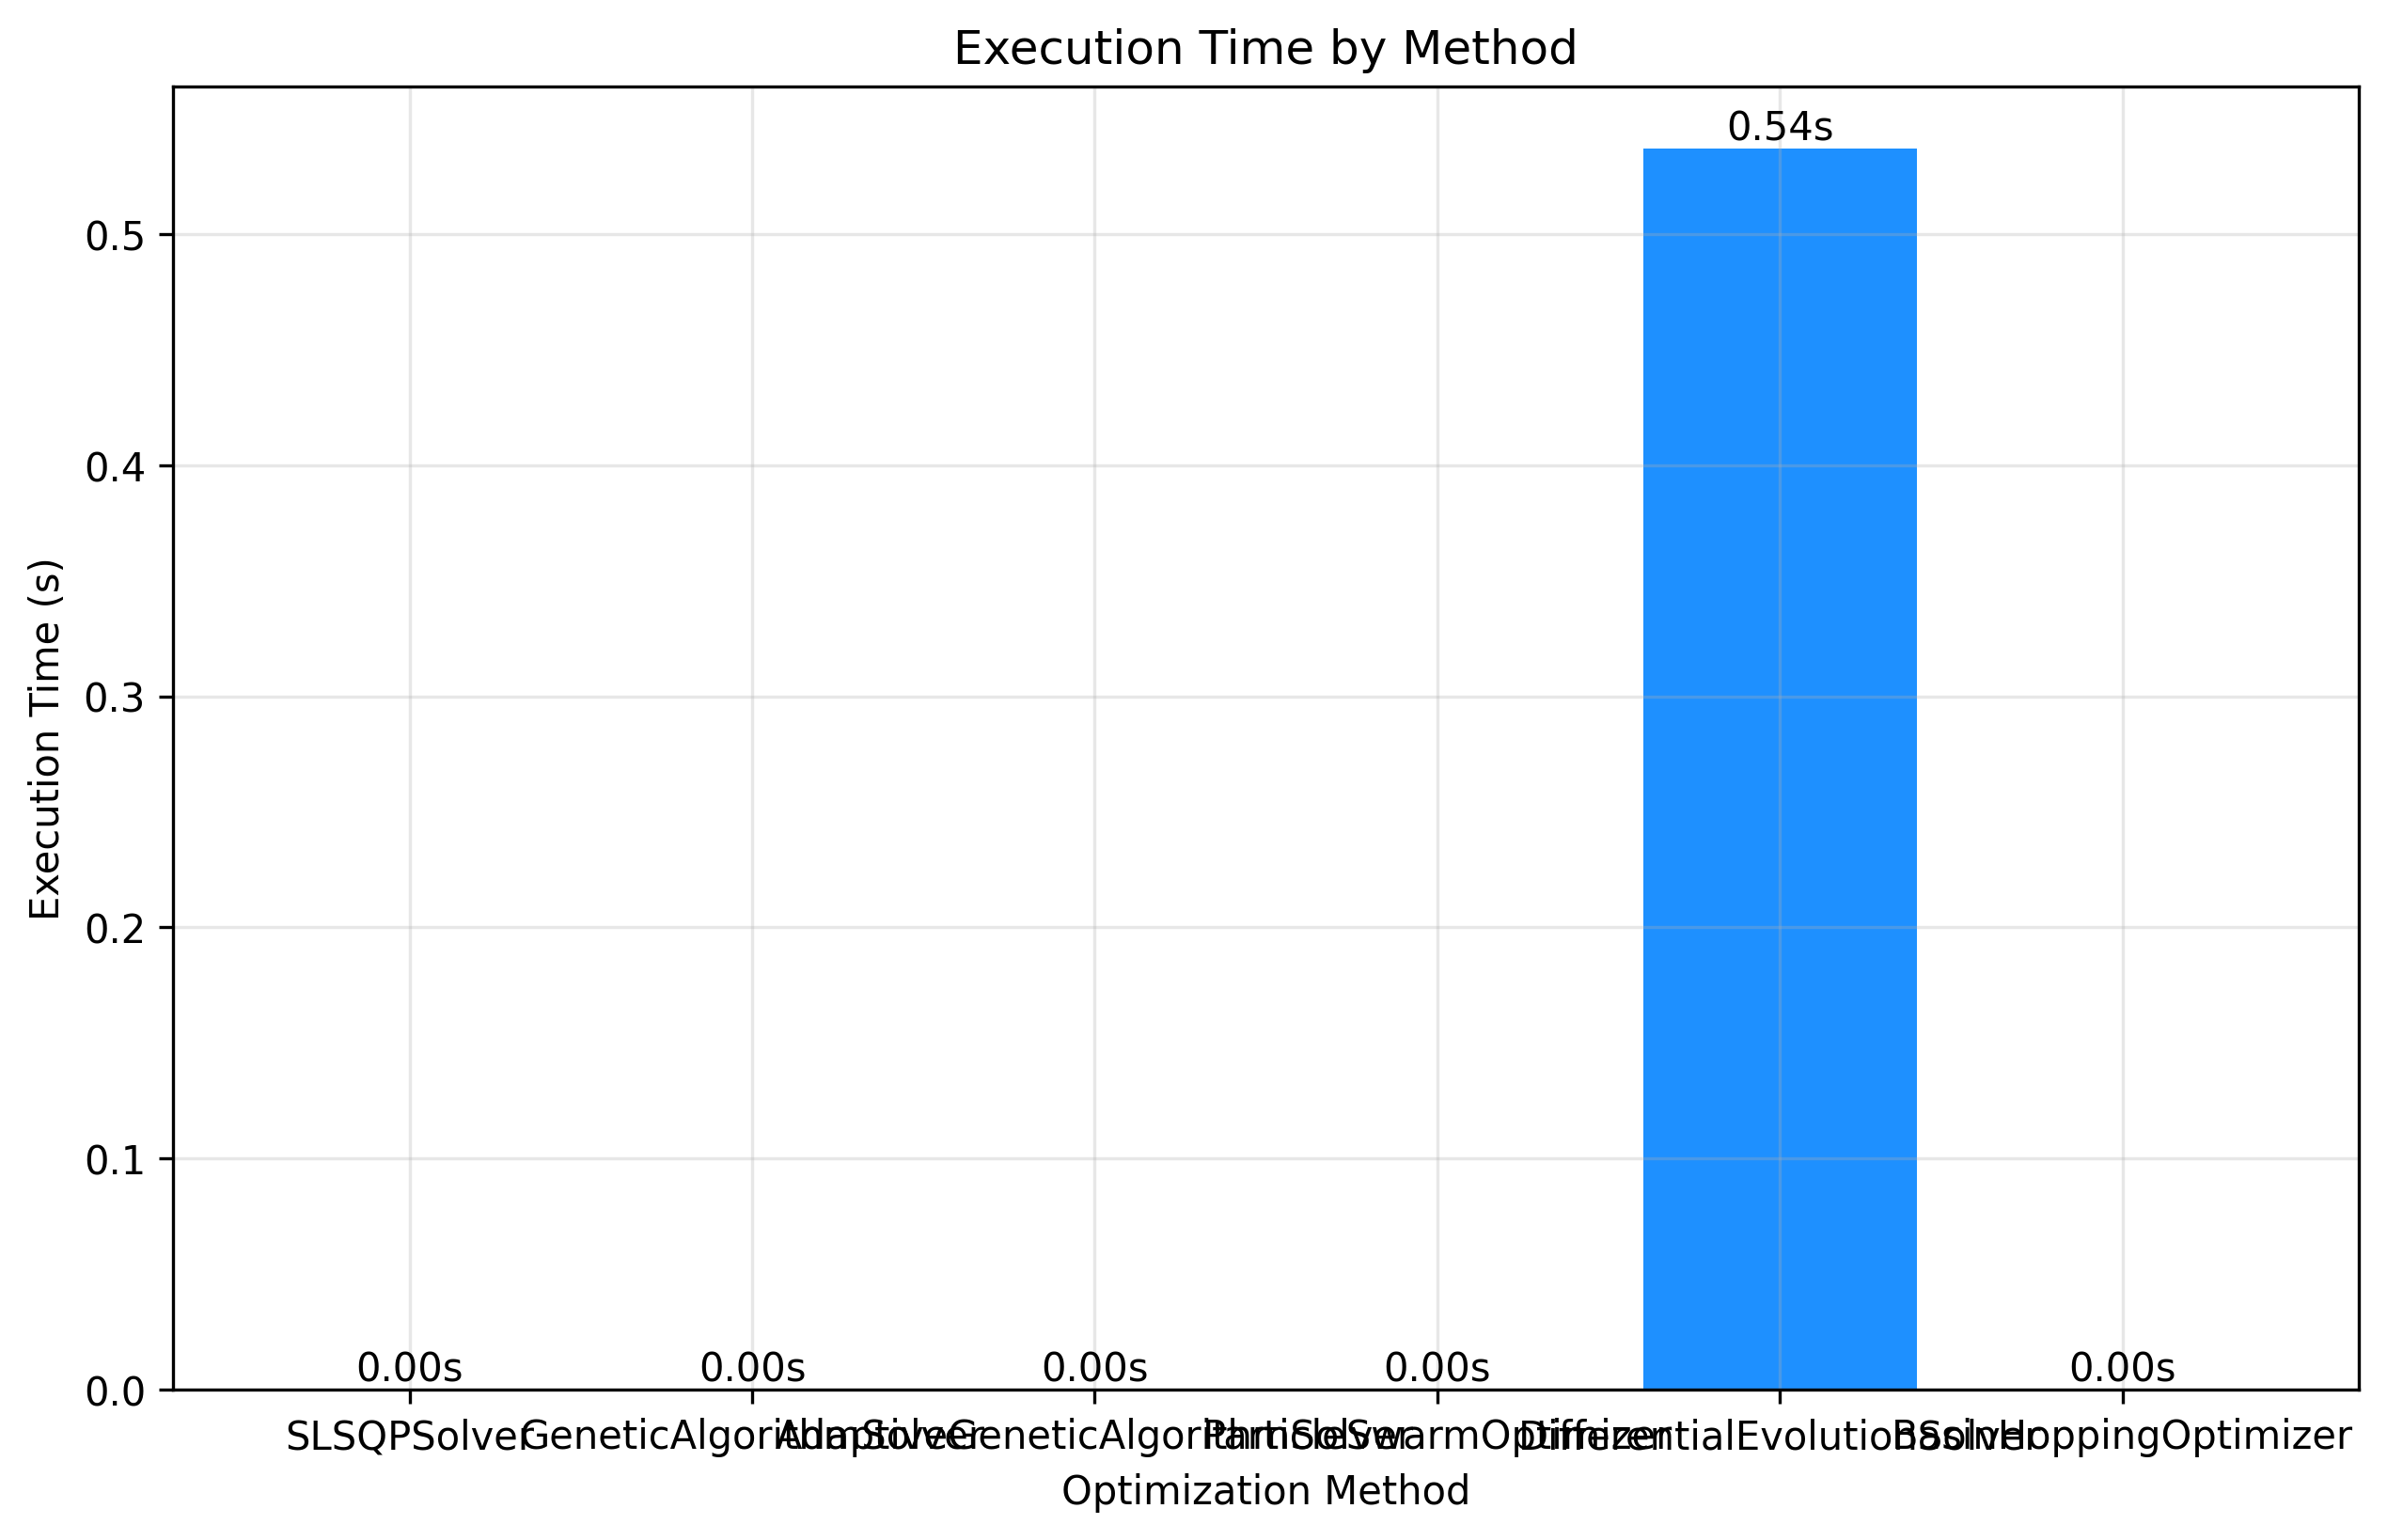
\includegraphics[width=\textwidth]{execution_time.png}
\caption{Execution time comparison between solvers}
\end{figure}

\subsection{Payload Fraction}
\begin{figure}[H]
\centering
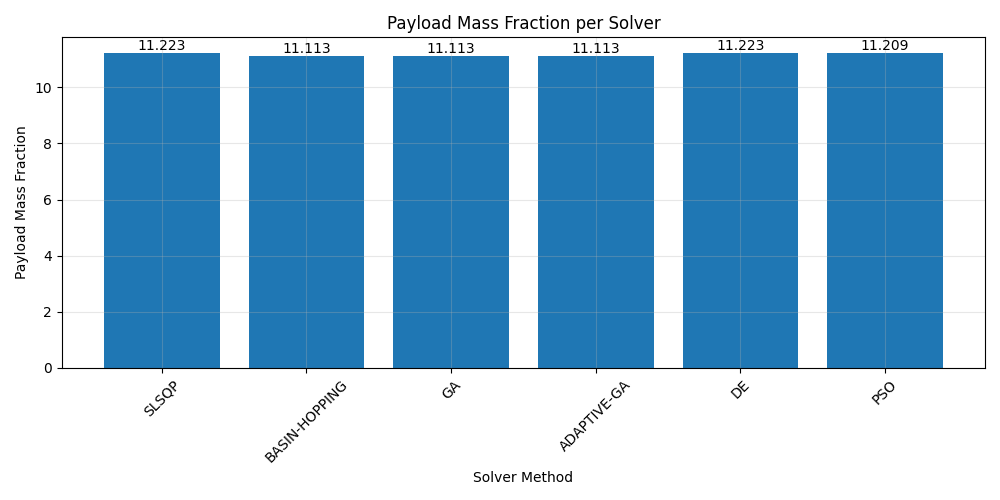
\includegraphics[width=\textwidth]{payload_fraction.png}
\caption{Payload fraction comparison between solvers}
\end{figure}

\subsection{Delta-V Breakdown}
\begin{figure}[H]
\centering
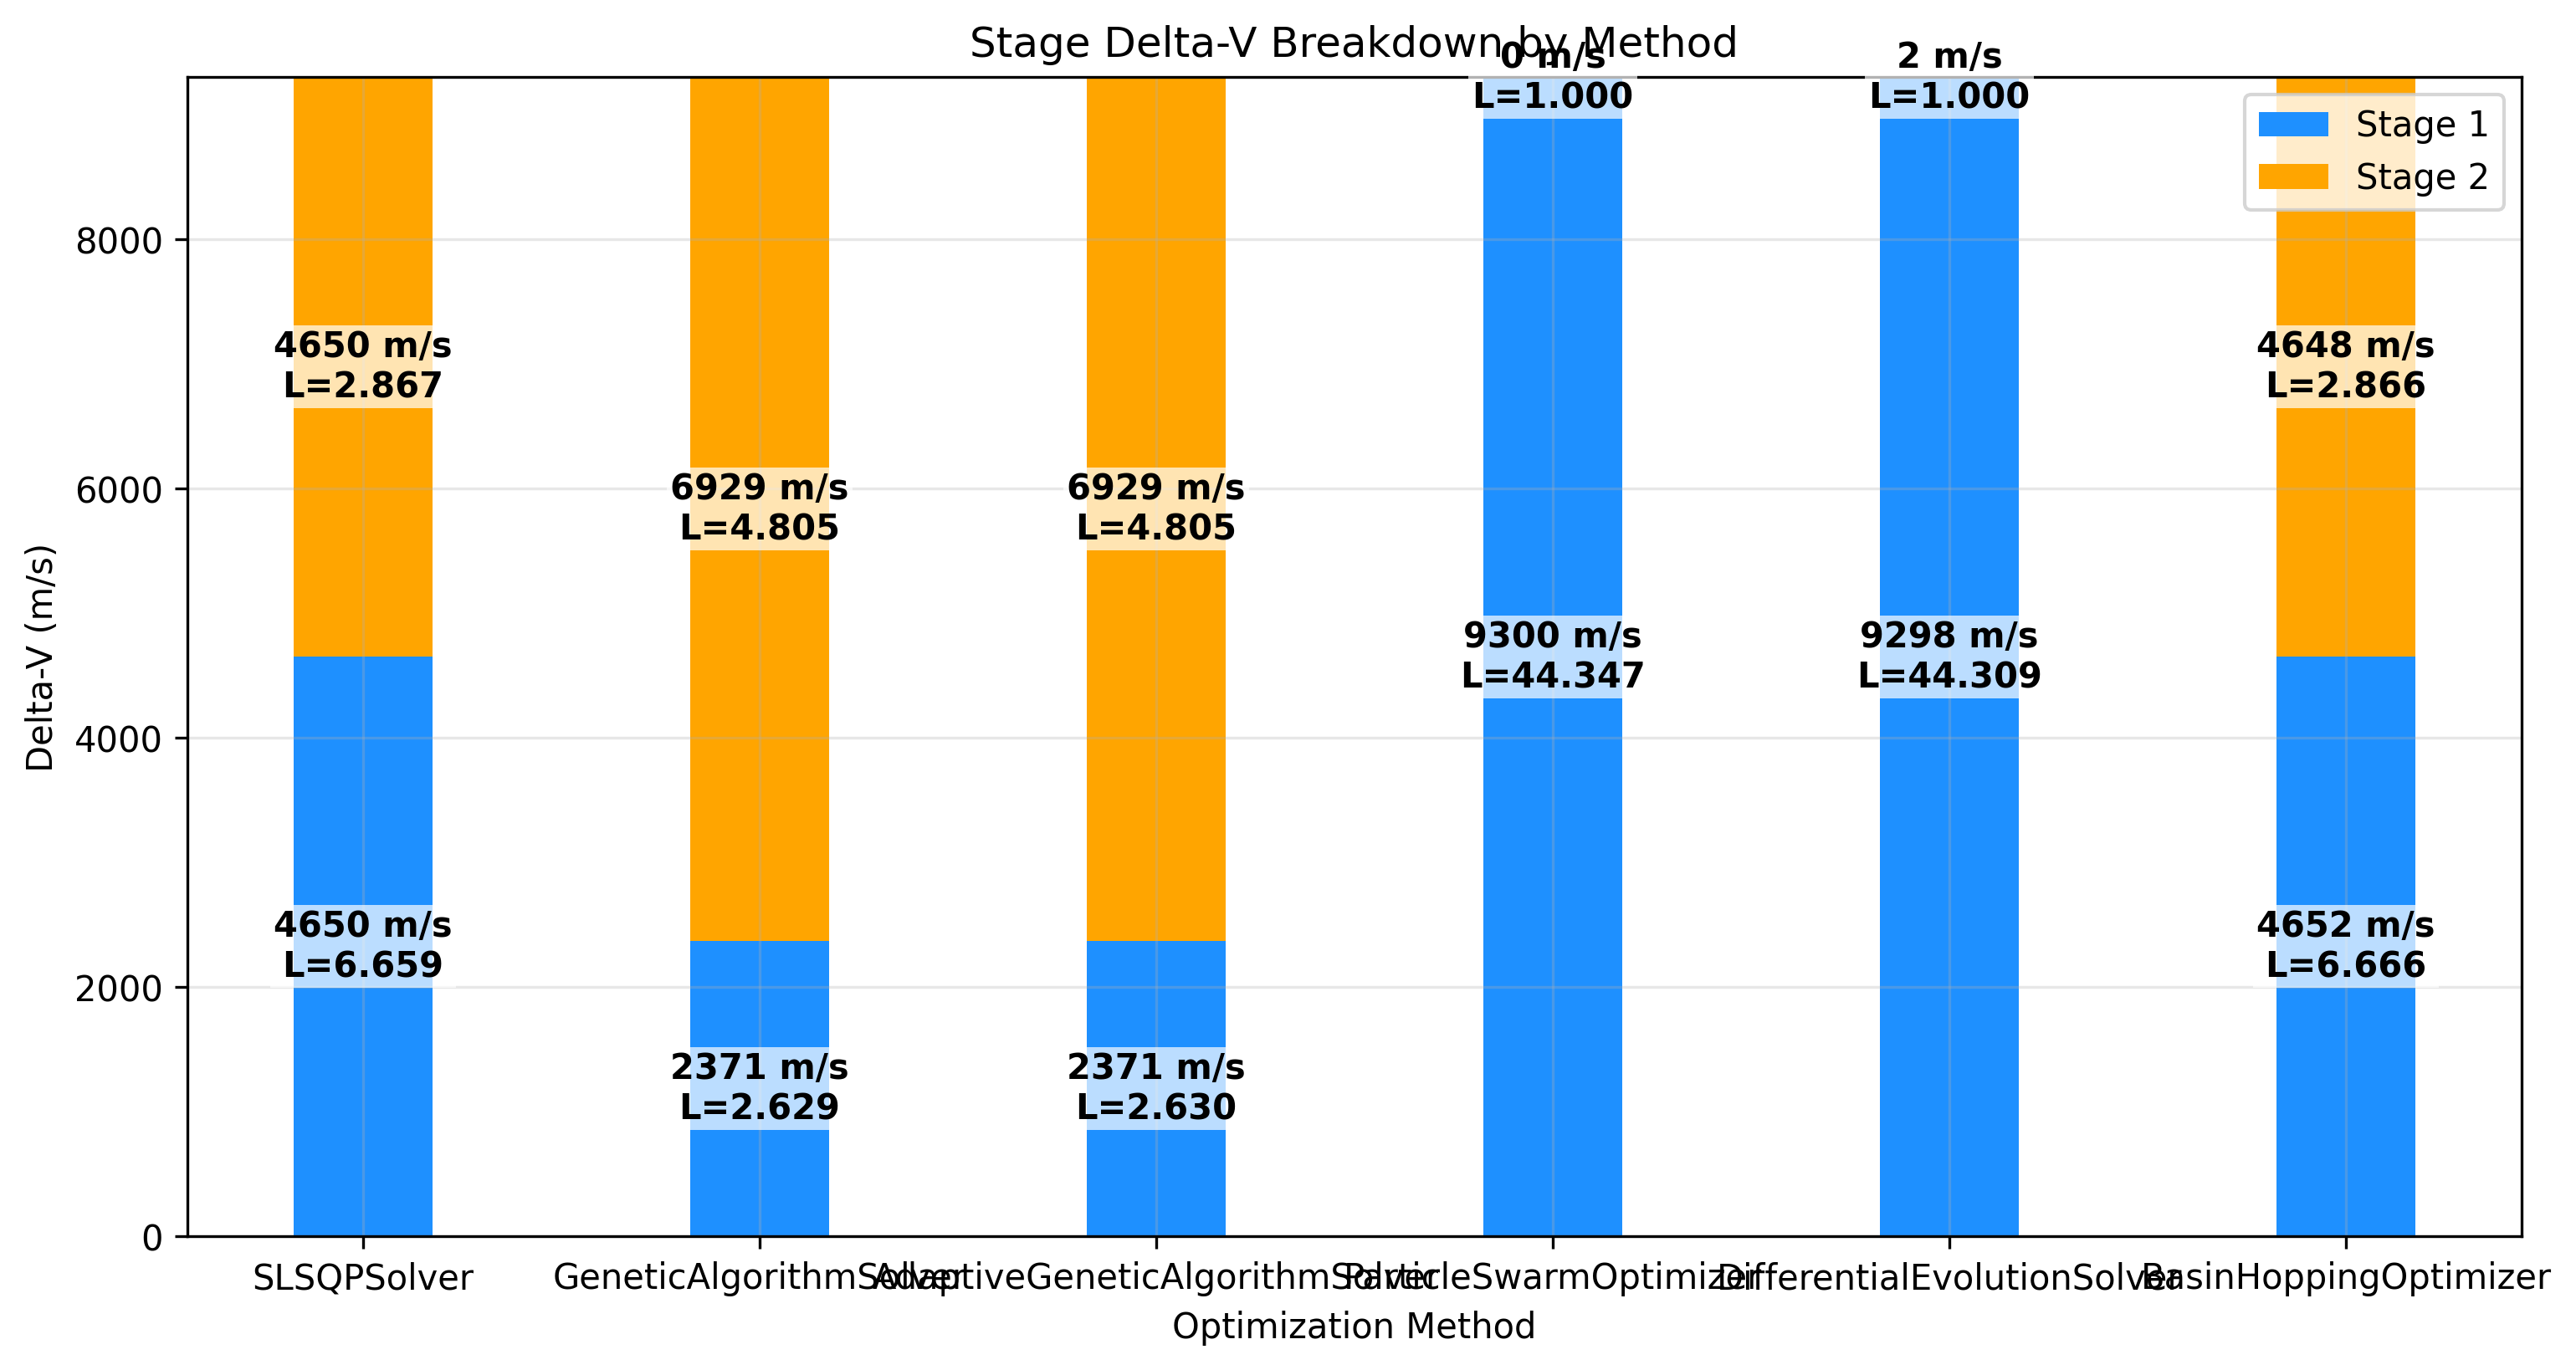
\includegraphics[width=\textwidth]{dv_breakdown.png}
\caption{Delta-V breakdown by solver}
\end{figure}

\section{Optimization Results}
\begin{table}[H]
\centering
\caption{Optimization Results by Solver}
\small
\begin{tabular}{lcccc}
\toprule
Method & Time (s) & Payload Fraction & $\Delta$V & Mass Ratio \\
\midrule
SLSQP & 0.002978 & 0.031548 & 4650.00, 4650.00 & 0.15, 0.22 \\
differential_evolution & 0.111281 & 0.035547 & 2773.01, 6526.99 & 0.33, 0.11 \\
BASIN-HOPPING & 0.199372 & 0.031550 & 4649.46, 4650.54 & 0.15, 0.22 \\
\bottomrule
\end{tabular}
\end{table}

\end{document}
